\documentclass{beamer}
\usepackage[autokw=all]{svn-multi}
\setbeamertemplate{navigation symbols}{}
%\usetheme{Goettingen}
\usetheme{Malmoe}
\usefonttheme{default}
%\setbeamersize{text margin left=5pt,text margin right=5pt}

\usepackage{hyperref}
\usepackage{subfigure}
\usepackage{amsmath}
\usepackage{amssymb}
\usepackage{multimedia}
\usepackage{shadow}
%\usepackage{movie15}

\usepackage{tcolorbox}

% Create a ``Wider'' command to reduce margins.  Put
% ``\Wider{\lipsum[2]}'' in a frame...
\newcommand\Wider[2][3em]{%
\makebox[\linewidth][c]{%
  \begin{minipage}{\dimexpr\textwidth+#1\relax}
  \raggedright#2
  \end{minipage}%
  }%
}


%\usepackage[english]{babel}
%\usepackage{pgf,pgfarrows,pgfnodes,pgfautomata,pgfheaps}
% \usepackage[latin1]{inputenc}

\usepackage{graphicx}
\defbeamertemplate*{footline}{default theme}
{
  \leavevmode%
  \hbox{%
  \begin{beamercolorbox}[wd=.5\paperwidth,ht=2.25ex,dp=1ex,center]{author in head/foot}%
    %\usebeamerfont{author in head/foot}\insertshortauthor~~(\insertshortinstitute)
    \usebeamerfont{author in head/foot}\insertshortauthor
  \end{beamercolorbox}%
  \begin{beamercolorbox}[wd=.4\paperwidth,ht=2.25ex,dp=1ex,center]{title in head/foot}%
    \usebeamerfont{title in head/foot}\insertshorttitle
  \end{beamercolorbox}%
  \begin{beamercolorbox}[wd=.1\paperwidth,ht=2.25ex,dp=1ex,right]{date in head/foot}%
%    \usebeamerfont{page number}\insertframenumber{} / \inserttotalframenumber\hspace*{2ex} 
    \usebeamerfont{page number}\insertpagenumber{} / \insertpresentationendpage{} \hspace*{2ex} 
  \end{beamercolorbox}}%
  \vskip0pt%
}

\title[Chronic Electrode Bundles]{Chronic Recording, Stimulation, and Steering Control with Electrode Bundles}

\author{Ben Pearre}
%\institute[]{
%  Computer Science\\
%  University of Colorado at Boulder, USA}
\date{\today}
%\date{\today}

\begin{document}

\begin{frame}
  \titlepage
\end{frame}

\begin{frame}
  \frametitle{Outline}
  \tableofcontents
\end{frame}


%\begin{frame}
%  \outline
%\end{frame}


\section{Introduction}
\subsection{Goals}

\begin{frame}
  \frametitle{Controlling behaviour with chronically implanted electrodes}
  \begin{itemize}
  \item Long-term stable recording
  \item Safe stimulation (despite small surface area)
    \vskip 0.6 cm
  \item Goal-directed modification of behaviour
    \begin{itemize}
    \item Optimise stimulation parameters
      \begin{itemize}
      \item Learn to produce desired output
      \item Safety constraints\dots
      \end{itemize}
    \end{itemize}
  \end{itemize}
\end{frame}


\subsection{Previous work}

\begin{frame}
  \frametitle{Pollo\dots Sch\"upbach [2014]}
  \begin{columns}
    \column{5cm}
    Slightly directional electrode
    \vskip 0.3 cm
    \includegraphics[width=\textwidth]{pollo1}
    \column{5cm}
    Finite element analysis
    \vskip 0.3 cm
    \includegraphics[width=\textwidth]{pollo2}
    
    \includegraphics[width=\textwidth]{pollo4}
  \end{columns}
\end{frame}


\begin{frame}
  \frametitle{Chaturvedia, Foutza, McIntyre [2015]}
  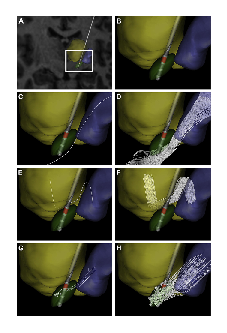
\includegraphics[width=0.35\textwidth]{chaturvedi-steering-0}
  
\includegraphics[width=0.3\textwidth]{chaturvedi-steering-1}
  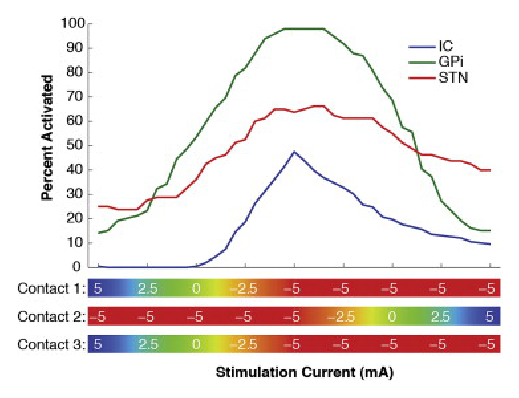
\includegraphics[width=0.3\textwidth]{chaturvedi-steering-2}
\end{frame}


\begin{frame}
  \frametitle{Previous work}
  \begin{description}
  \item[Current Steering] using finite element analysis
    \begin{itemize}
    \item Faster than hand-tuning
    \item Some success
    \item Coarse-grained
    \item All models are wrong.  Some models are useful.
    \end{itemize}
  \item[Recording] for ``closed-loop'' therapy
    \begin{itemize}
    \item Large populations
    \item Good luck
    \end{itemize}
  \end{description}
\end{frame}



\section{Materials}
\subsection{Electrodes}

\begin{frame}
  \frametitle{Electrodes}
  \begin{columns}
    \column{4cm}
    Chronic high-count high-impedance\dots
    \begin{itemize}
    \item Carbon fibres
    \item Silicon carbide
    \item Optical\dots?
    \end{itemize}
    \column{7cm}
    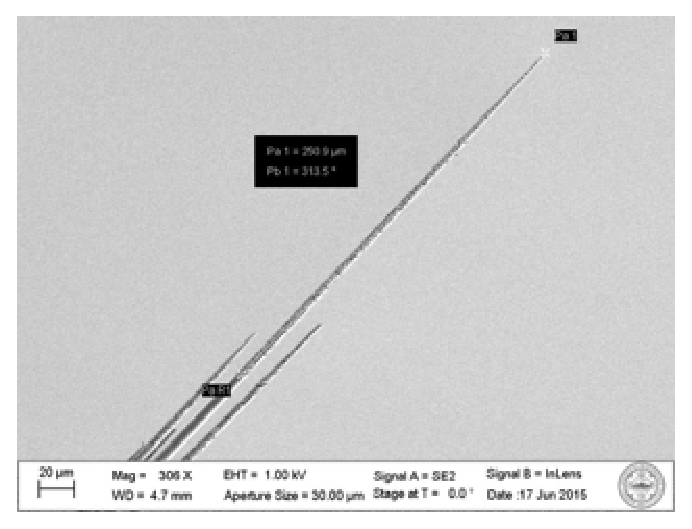
\includegraphics[width=\textwidth]{electrodes_up_close}
  \end{columns}
\end{frame}

\begin{frame}[plain]
  \begin{center}
    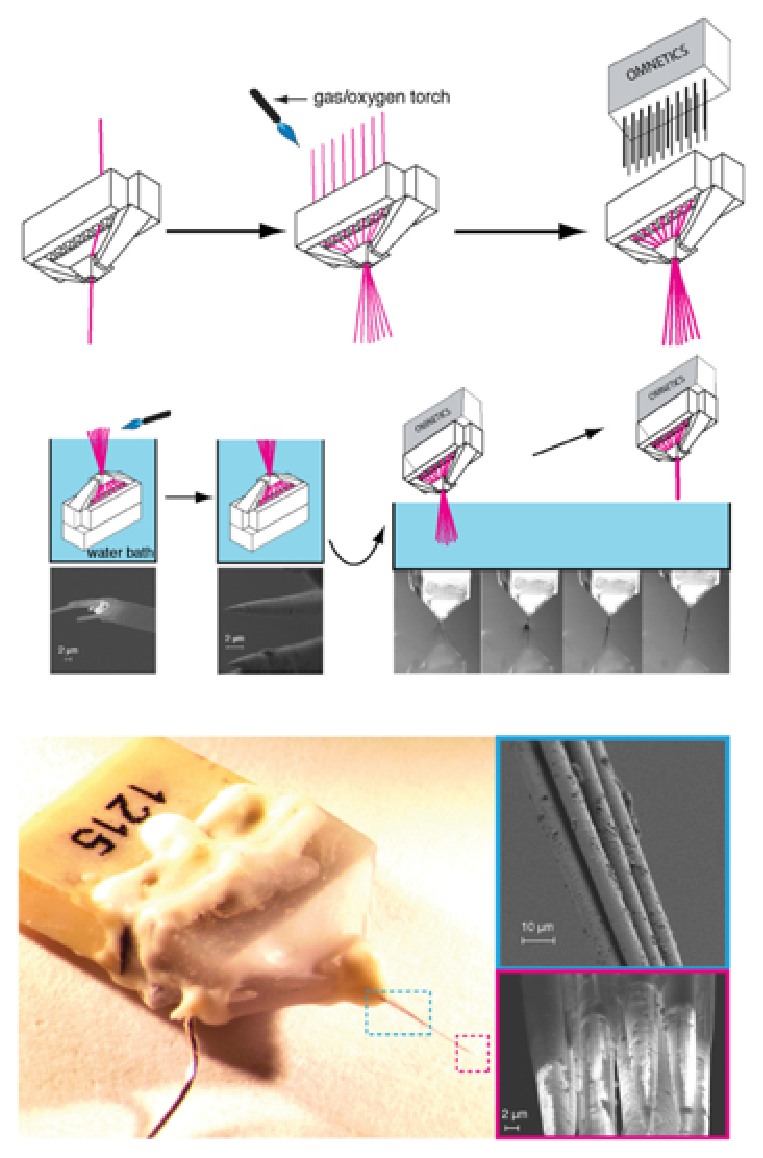
\includegraphics[height=\textheight]{julia_electrodes}
  \end{center}
\end{frame}

\begin{frame}
  \begin{center}
  \includegraphics[height=0.9\textheight]{CFHistSplayFronSanneImg1}
  \includegraphics[height=0.9\textheight]{CFHistSplayFronSanneImg2}
  \end{center}
\end{frame}

\subsection{Stimulator}

\begin{frame}
  \frametitle{Plexon stimulator}
  \begin{itemize}
    \item 16 channels
    \item Current-controlled
    \item Externally triggered
    \item Arbitrary pulse waveforms
    \item Resolution: 30 nA $\times 1 \mu$s
    \item Matlab API
    \item Reprogramming time $\approx$ 0.2s/channel
    \item Voltage monitoring is expensive!
  \end{itemize}
\end{frame}



\section{Experiments}

\subsection{Chronic recording}

\begin{frame}
  \frametitle{Recording --- bare carbon in X}
  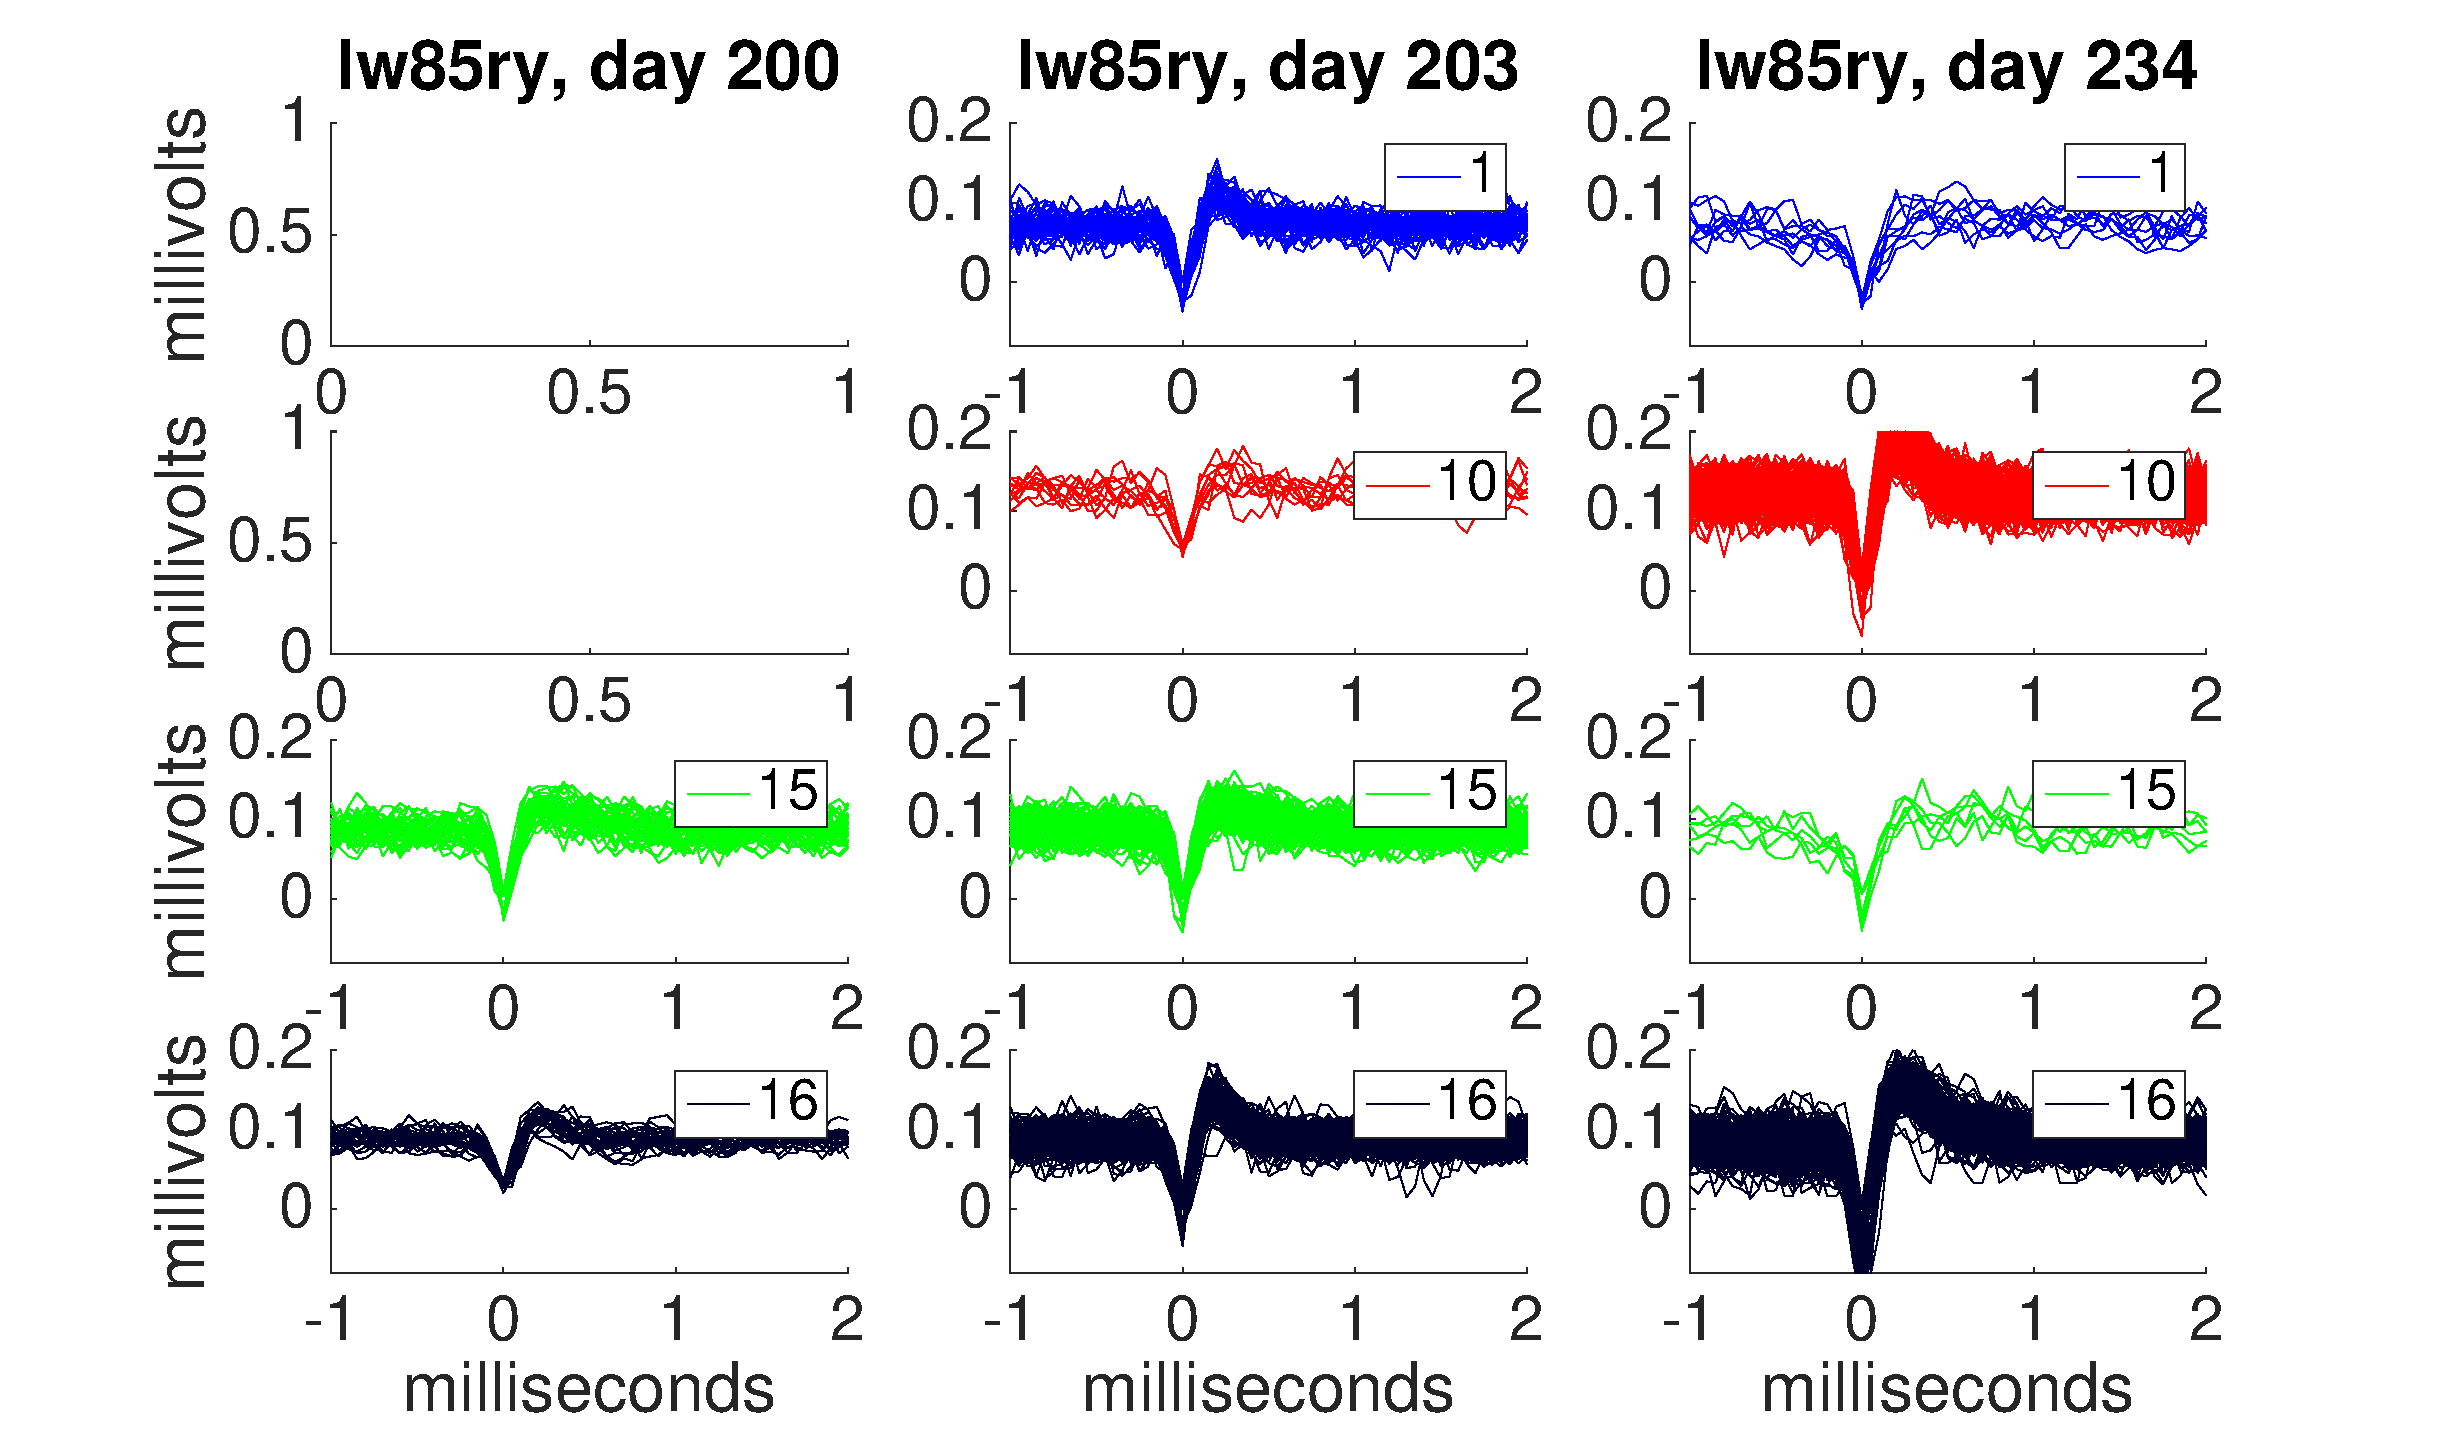
\includegraphics[width=\textwidth]{lw85ry_several}
\end{frame}

\begin{frame}
  \frametitle{Questionable recording --- IrO$\textsubscript{2}$ in X}
  \includegraphics<1>[width=\textwidth]{spiketrain-lw95rhp-2015-11-19}
  
  \includegraphics<1>[width=\textwidth]{spiketrain-lw95rhp-2015-11-23}
  \includegraphics<2>[width=\textwidth]{lw95rhp_several}
\end{frame}


\subsection{Stimulation}


\begin{frame}
  \frametitle{Antedromic HVC $\leftarrow$ X response}
  \begin{center}
  \includegraphics<+>[width=0.8\textwidth]{hvc_areaX}
  \includegraphics<+>[width=0.95\textwidth]{plexme}
  \end{center}
\end{frame}




\subsection{Current Steering}


\begin{frame}
  \frametitle{Combinatorial optimisation}
  \begin{columns}
    \column{5 cm}
    \begin{center}
      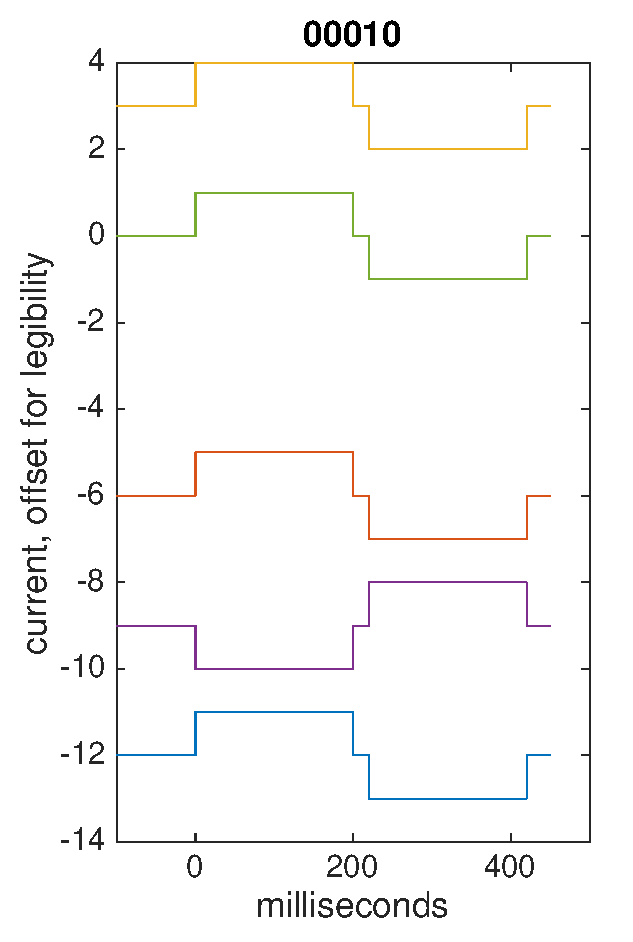
\includegraphics[width=0.8\textwidth]{pulsedemo1}
    \end{center}
    \column{5 cm}
    \begin{center}
      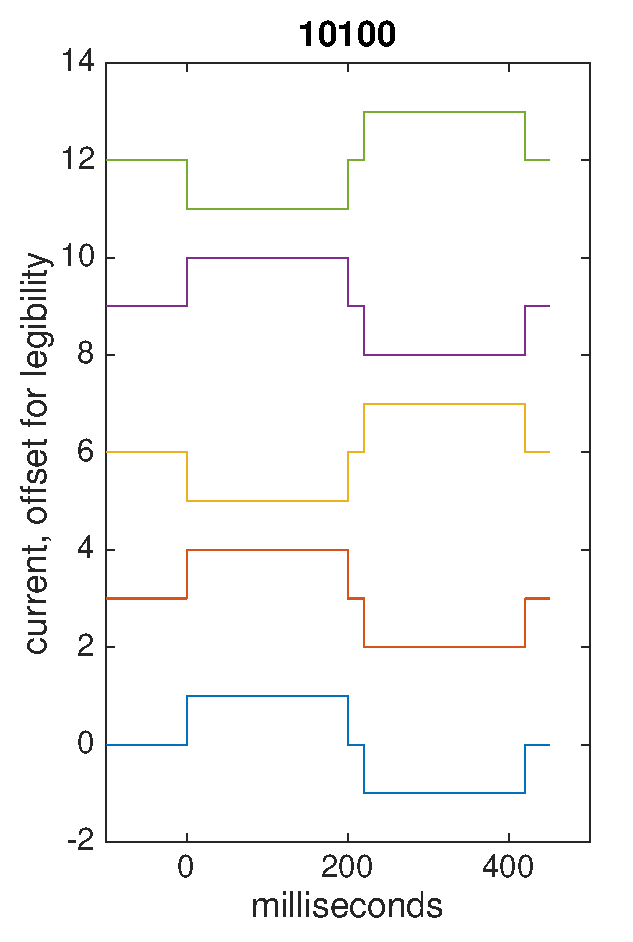
\includegraphics[width=0.8\textwidth]{pulsedemo}
    \end{center}
  \end{columns}
\end{frame}

\begin{frame}
  \frametitle{Combinatorial optimisation}
  \includegraphics[width=0.95\textwidth]{plexme}
\end{frame}

\begin{frame}
  \frametitle{Combinatorial optimisation}
  Can current steering minimise stimulation voltage?
  \begin{enumerate}
  \item Pick a current-steering configuration
  \item Find response threshold
  \item Check each channel for voltage
  \end{enumerate}
\end{frame}


\begin{frame}
  \frametitle{Voltage minimisation}
  \includegraphics<+>[width=\textwidth]{current_steering_voltages}
  \includegraphics<+>[width=\textwidth]{current_steering_voltages_valid}
\end{frame}




\begin{frame}
  \frametitle{Response shaping in HVC}
  \begin{center}
    \includegraphics[width=\textwidth]{current-steering-hvc}
  \end{center}
\end{frame}





%%% Future! %%%
\section{The Future!}
\subsection{Ideas}

\begin{frame}
  \frametitle{Policy optimisation}
  \begin{columns}
    \column{35mm}
    {\bf Criteria}
    \begin{itemize}
      \item See response
      \item Maximise response
      \item Minimise voltage
      \item Separate responses
      \item Directed change to song
        \begin{itemize}
          \item Acute
          \item Chronic
        \end{itemize}
    \end{itemize}
    \column{35mm}
    {\bf Policy outputs}
    \begin{itemize}
      \item Pulse train timing
      \item Channel timing
      \item Arbitrary pulse shape
        \vskip 0.5 cm  \item {\em Optical!}

    \end{itemize}
    \column{35mm}
    {\bf Policy inputs}
    \begin{itemize}
      \item Vocalisation
      \item Neural activity
      \item Other motor output?
    \end{itemize}
  \end{columns}
\end{frame}


\subsection{Electrodes}
\begin{frame}
  \includegraphics<+>[width=\textwidth]{stuart}
\end{frame}



\subsection{Optimisation}

\begin{frame}[label=appendixeR]
  \frametitle{Gradient estimation: eR / Stochastic Approximation}
  \begin{description}
  \item[Policy:]
    \[
    \pi(s,u;\theta) = \Pr(u|s;\theta)
    \]
  \item[Gradient:]
    \[
    \widehat{\nabla_\theta J(\theta)} = \widehat{g_\theta} = \left< \left( \sum_{k=0}^H
    \nabla_\theta \log\Pr(u_k|s_k;\theta)\right) \cdot (r-b)\right>
    \]
  \item[Learning:]
    \[
    \theta_{e+1} = \theta_e+\alpha\frac{\nabla_\theta
      J(\theta)}{\left|\nabla_\theta J(\theta)\right|}
    \]
  \end{description}
\end{frame}

\begin{frame}
  \frametitle{Gradient estimation: eR / Stochastic Approximation}% \hfill\hyperlink{eR<5>}{\beamerreturnbutton{}}}
  \begin{description}
  \item[Reward:]
    \[
    %r = -d
    r(d,m)=-\left(d+\eta\sum_{j=1}^n\left(\max\left[0,\;\;\left(\frac{\mu D}{m_j}\right)^2-1\right]\right)\right)
%r(d,m)=-\left(d^2+\eta\left(\max\left(\left(\frac{\mu      D}{m}\right)^2-1, \; \; 0\right)\right)\right)
    \]
  \item[Eligibility:]
    \begin{eqnarray*}
      u &=& \theta + {\cal N}(0, \Sigma)\\
      %\Pr(u|s;\theta) &=& \frac{1}{(2\pi)^\frac{N}{2}\sqrt{(|\Sigma|)}}
      %\exp\left(-\frac{(u-\theta)^T\Sigma^{-1}(u-\theta)}{2}\right)\\
      \nabla_\theta\log\Pr(u|s;\theta) &=& \frac{1}{2}\left(
      \Sigma^{-1}+\Sigma^{-1\,T} \right) \left( u - \theta \right)
    \end{eqnarray*}
  \end{description}
\end{frame}

\end{document}
